% ============================================================
% Course Report Template
% DO NOT EDIT THIS FILE (except the metadata block below).
% Write your content in the sections/ folder.
% ============================================================
\documentclass[10pt,twocolumn]{article}

% ---------- Packages ----------
\usepackage[margin=0.75in]{geometry}
\usepackage{times}              % Serif font (conference standard)
\usepackage{graphicx}           % Figures
\usepackage{amsmath,amssymb}    % Math
\usepackage{cite}               % IEEE-style citation sorting
\usepackage{hyperref}           % Clickable references
\usepackage{booktabs}           % Better tables
\usepackage{caption}            % Caption formatting
\usepackage{fancyhdr}           % Custom headers/footers
\usepackage{lipsum}             % Placeholder text (remove in final)
\usepackage{coursemacros}       % Course-specific commands
\usepackage{cleveref}           % auto "Table"/"Figure" in references
\usepackage{pdflscape}
\usepackage{siunitx}

% ============================================================
% STUDENTS: FILL IN THIS SECTION
% ============================================================
\newcommand{\reporttitle}{Cycle-Accurate Simulator for Atalla Ax01 Performance Analysis}
\newcommand{\coursesemester}{Spring 2026}

% Register each team member: \addauthor{Name}{email}{\coursenum or \coursenumgrad}
% 2 students per line.
\addauthor{Rafael Monteiro Martins Pinheiro}{rmontei@purdue.edu}{\coursenumsdfirst}

% ============================================================

% ---------- Hyperref setup ----------
\hypersetup{
    colorlinks=true,
    linkcolor=blue,
    citecolor=blue,
    urlcolor=blue,
}

% ---------- Caption styling ----------
\captionsetup{font=small, labelfont=bf}

% ---------- Footer with author names + page numbers ----------
\pagestyle{fancy}
\fancyhf{}                          % clear all headers/footers
\renewcommand{\headrulewidth}{0pt}  % no header line
\fancyfoot[L]{\small \authorlist}
\fancyfoot[R]{\small \thepage}

% ============================================================
\begin{document}

% ---------- Cover Page (single-column) ----------
\onecolumn
\thispagestyle{empty}
\vspace*{\fill}
\begin{center}
    {\LARGE\bfseries \reporttitle \par}
    \vspace{1.5cm}
    {\large
    \begin{minipage}{0.9\textwidth}
        \centering
        \authorblock
    \end{minipage}
    \par}
    \vspace{1cm}
    {\large \coursesemester \par}
    \vspace{1.5cm}
    {\large The feedback for the report is to be returned to: \par}
    \vspace{0.5cm}
    {\large Rafael Monteiro Martins Pinheiro \par}
    {\large rmontei@purdue.edu \par}
    \vspace{1cm}

    {\large This project was mentored by the following Teaching Assistants: \par}
    \vspace{0.5cm}
    {\large Akshath Raghav Ravikiran, araviki@purdue.edu \par}
    {\large Sooraj Chetput Venkataraghavan, schetput@purdue.edu \par}

\end{center}
\vspace*{\fill}
\newpage

% ---------- Body begins (two-column with spanning title) ----------
\twocolumn[%
    \begin{center}
        {\Large\bfseries \reporttitle \par}
        \vspace{0.3cm}
        {\normalsize \authorblock \par}
        \vspace{0.5cm}
    \end{center}
]
\setcounter{page}{1}  % restart numbering after cover
\thispagestyle{fancy} % ensure footer appears on first body page

% ---------- Abstract ----------
\begin{abstract}
% Paste your abstract here (no \begin{abstract} needed — main.tex handles that).
Semiconductor product development proceeds from high-level design to physical implementation, with RTL serving as a critical but resource-intensive stage where design errors significantly increase cost and risk. This challenge is amplified in AI accelerators, where aggressive throughput targets and complex data movement strategies increase design and verification complexity.

Atalla is a domain-specific AI accelerator targeting tensor workloads, with a focus on efficient General Matrix Multiplication (GEMM) and optimized data movement. To enable early design-space exploration prior to RTL completion, we develop Atalla-Sim, a custom Python-based, cycle-level simulator that validates functional correctness against PyTorch GEMM golden models while supporting performance analysis and microarchitectural optimization. By modeling pipeline behavior, execution timing, and data movement at cycle granularity, Atalla-Sim enables systematic evaluation of design tradeoffs and quantification of their performance impact before hardware implementation.

We implement a modular simulation infrastructure and validate key components to support pre-silicon studies and hardware–software integration testing. Our results demonstrate the ability to perform early design-space exploration and reduce integration risk. Although currently limited in performance on large workloads compared to C++-based frameworks, Atalla-Sim establishes a foundation for scaling to broader workloads, faster validation, and more informed design decisions.

\end{abstract}

% ---------- Body ----------
\section{Background}
% Relevant background.
% Cite prior work using \cite{key} — entries go in references.bib.
\subsection{Motivation on Deep Neural Network Accelerators and the development of the Atalla}
For decades, the dominant paradigm in applied computing rested on expert-designed, hand-crafted heuristics, an approach fundamentally inadequate for real-world complexity, as hand-written rules cannot generalize gracefully. The emergence of Deep Neural Networks (DNNs) represents a decisive shift: a single general-purpose learning program that autonomously extracts hierarchical representations from raw data, recognizing patterns at multiple levels of abstraction without explicit human specification \cite{efficientprocessingofdnn}.

However, the superior accuracy of DNNs comes at the cost of high computational complexity \cite{efficientprocessingofdnn}. The breakdown of Dennard Scaling and the deceleration of Moore's Law, from a doubling of compute performance every 18 months to once every 20 years, have ruled out the expectation that general-purpose hardware will keep pace. This was made economically tangible at Google, where internal analysis found that just three minutes of daily DNN-based voice search per Android user would necessitate doubling the company's entire data center footprint—a capital investment deemed unsound. The response was a decisive industry pivot toward Domain-Specific Architectures (DSAs): circuits designed to perform a narrow subset of tasks with extreme efficiency \cite{pattersontpulecture}.

\begin{figure}
    \centering
    \includegraphics[width=1\linewidth]{figures/dnngemm.png}
    \caption{GEMM modelling of a DNN layer}
    \label{fig:dnngemm}
\end{figure}

AI accelerators are DSAs specialized for the dominant ML kernels, such as General Matrix Multiplications (GEMMs) and Convolutions (CONVs), employing a systolic array compute fabric: a 2D grid of processing elements (PEs) that passes inputs horizontally and partial sums vertically, maximizing data reuse and minimizing costly off-chip memory accesses \cite{scpadfinalreport}. The Atalla Ax01 \cite{atallasite} is grounded in this same logic, and understanding its architecture requires appreciating this broader convergence of algorithmic necessity, physical scaling limits, and market drive \cite{pattersontpulecture}.

\subsection{Need for Hardware Simulation}

While analytical performance models offer a quick mean of estimating hardware behavior, they are insufficient for evaluating modern architectures. The sheer number of configurations, pipeline interlocks, memory access patterns, and microarchitectural corner cases that affect real performance cannot be faithfully captured by closed-form formulas. Implementation details produce significant and non-obvious performance variations that only come up under realistic workload conditions. Simulation has consequently become the industry standard performance modeling method prior to committing to silicon \cite{surveycomparchsim}.

The most manageable simulation methodology for complex hardware is Discrete-Event Simulation (DES), which models system progression through an event scheduler and queue rather than advancing time cycle-by-cycle through idle states \cite{surveycomparchsim}. DES is formally expressed through Petri Nets, in which hardware is abstracted into three primitives:

1- tokens: serve as abstraction of carriers of information, such as instructions or data packets,

2- places: represent storage entities such as registers and buffers, and

3- transitions: model processing models such as ALUs and arbiters.

A transition fires when its input places hold sufficient tokens, consuming them and producing output tokens, capturing the data-driven, concurrent behavior of pipelined hardware \cite{casvliw}.

Translating architectural intent into Register-Transfer Level (RTL) remains a "mammoth task". Functional verification alone routinely demands tens or hundreds of person-years of engineering effort and substantial compute infrastructure, yet nearly 50\% of chips require additional unplanned tape-outs due to functional bugs that escaped pre-silicon verification, leading to financial and scheduling penalties. Software simulations mitigate this risk by serving as a functional correctness tool by providing a behavioral reference for which against RTL can be validated much more easily than dense tenstbenches \cite{unifiedmethpresiverif}.

Consolidated simulation infrastructures such as gem5 illustrate the maturity of this discipline, representing over 20 years of collaborative development between more than 250 contributors and 7,000 commits. This accumulated investment makes simulation a bedrock for hardware-software co-design, enabling design space exploration and software stack validation long before tape-out, thereby reducing time-to-market and integration risk \cite{gem5}.
% Subsection: Motivation on DNN accelerators
% Quick history on the TPU for motivating AI accelerators
% https://www.youtube.com/watch?v=fhHAArxwzvQ&t=2626s -- 9:49
% Why are we building Atalla -- https://purdue-socet.github.io/atalla/overview.html

% Subsection: Simulation
% Discre-event simulators work
% Why do we need simulators
% Look at papers that reference gem5, gpgpu-sim -- industry needs simulators because RTL design is time consuming and needs workforce

\section{Introduction}
% Introduce the problem, motivation, and relevant background.
% Cite prior work using \cite{key} — entries go in references.bib.

% Subsection 1: Atalla top-level
% Systolic Array
% Memory subsystem
% Vector core
% Scheduler
\subsection{Atalla Top-Level Architecture}

At the heart of the architecture is a 32x32 systolic array of PEs operating under a weight-stationary dataflow. In this regime, filter weights are latched whithin each PE across multiple input activations, maximizing weight reuse and minimizing the energy cost of repeated memory fetches: the dominant source of power dissipation in matrix-intensive workloads \cite{efficientprocessingofdnn, sysarrfinalreport}.

Surrounding this compute fabric is a 2 MB software-controlled Scratchpad memory that replaces conventional hardware-managed caches with explicit, programmer-directed data movement. A tile-descriptor based direct memory acces (DMA) engine orchestrates bulk transfers between off-chip DRAM and the Scratchpad, while a bank-swizzling scheme permutes address mapping across memory banks to eliminate bank conflicts during wide vector accesses characteristic of GEMM tiling \cite{scpadfinalreport}.

Interfacing between the Scratchpad and the systolic array is a 32-wide Vector Core, a datapath responsible for managing data-level parallelism (DLP) accross the full width of the array. The Vector Core communicates with the systolic array through the Global Systolic Array Unit (GSAU), which coordinates activation feeding, weight loading and result extraction; and it communicates with the Scratchpad through the Vector Load Store (VLS) unit (or VLSU), sending reads and write requests \cite{vcfinalreport}.

A 4-wide Very Long Instruction Word (VLIW) scheduler orchestrates all functional units (FUs) by issuing instruction bundles each cycle and managing inter-bundle data dependencies statically \cite{schedulerfinalreport}. By delegating the complexity of parallelism detection from hardware to the compiler, the architecture significantly simplifies the control logic and reduces power overhead compared to superscalar designs \cite{simplevliw}.

% Subsection 2: Custom ISA
% What is our ISA
% Why do we use it, instead of RISCV + extensions
% Why this is a barrier from using established simulators
\subsection{Custom Instruction Set Architecture Rationale and Simulation Challenges}

\begin{figure}
    \centering
    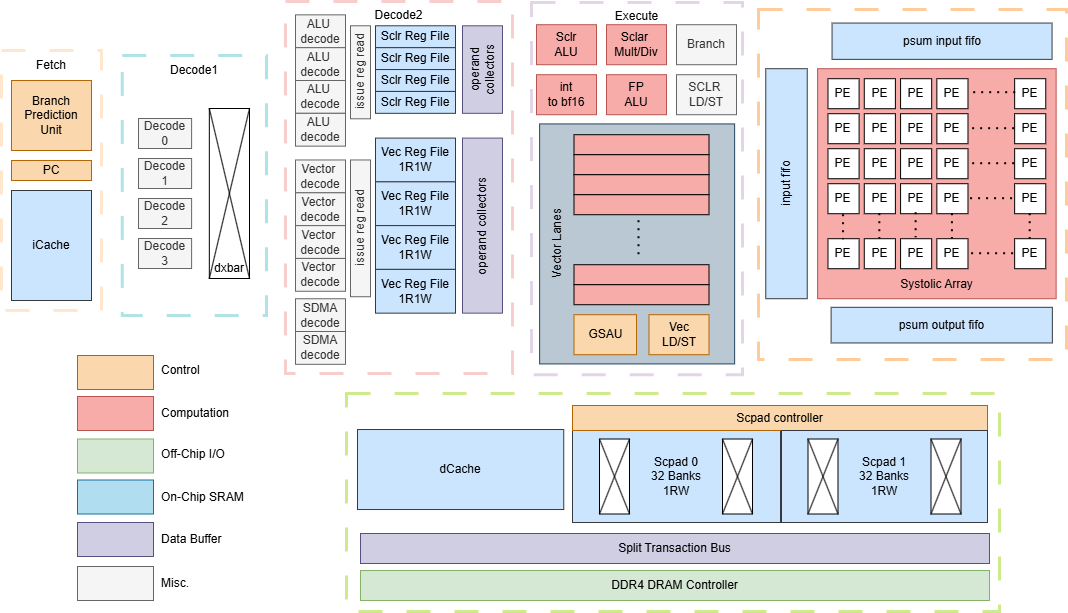
\includegraphics[width=1\linewidth]{figures/toplevelatalla-new.drawio.png}
    \caption{Atalla Ax01 Top-Level}
    \label{fig:toplevelatalla}
\end{figure}

Atalla utilizes a custom 40-bit Instruction Set Architecture (ISA) specifically optimized for tile-centric computing kernels. The ISA incorporates specialized instructions such as \texttt{gemm.vv} for initiating systolic array computations and \texttt{sdma} for orchestrating Scratchpad tile transfers \cite{sysarrfinalreport}. The design eliminates translation overhead and complex decode stades inherent in general-purpose architectures by mapping instructions directly to microarchitectural resources \cite{scpadfinalreport}. Standard alternatives like RISC-V Vector (RVV) introduce significant hardware bloat for domain-specific workloads by including support for Select Element Width (SEW), Extended Effective Width (EEW) and Length Multiplier (LMUL). These mandatory provisions require additional control logic and silicon area to support generality that is not exercised in an characterized AI accelerator  \cite{vcfinalreport, riscv, rvv}. A GEMM-native ISA allows the instruction encoding budget to be focused on high-throughput operations, resulting in a denser instruction stream and reduced decoder complexity \cite{sysarrfinalreport}.

In contrast, Atalla-Sim functions as a bespoke, functional validation framework by simulating Atalla’s Scratchpad traffic, vector datapath and systolic-array execution directly, bypassing the rigid front-end assumptions and legacy maintenance burden of general-purpose ISA simulators \cite{simplevliw}. Because it is specialized to handle the accelerator’s packetized, tile-oriented execution model, which requires modeling bonded "instruction lines" rather than the independent instruction tokens found in conventional superscalar engines, it can be adapted rapidly as the ISA and microarchitecture evolve \cite{casvliw}. This agility allows the simulator to serve as a critical tool for validating architectural intent and functional correctness against the hardware specification before the RTL is finalized. The cycle-accurate software environment complements rather than replaces RTL verification, providing a strong foundation for pre-silicon studies while acknowledging that RTL design remains a resource-intensive "mammoth task" \cite{unifiedmethpresiverif}.

As a result, an existing simulator cannot be used off the shelf to execute Atalla programs. Supporting the ISA would require implementing a new decoder for the 40-bit instruction format, defining the semantics of custom operations, and modeling accelerator-specific structures such as the scratchpad and systolic-array control path. These additions are substantial enough that the simulator would effectively need to be extended into a custom architectural model. For this reason, a purpose-built simulator is a more practical vehicle for functional validation of the Atalla ISA and its software stack.

% Subsection 3: VLIW
% What is VLIW
% Why is Atalla VLIW
% Previous work on VLIW simulation
% Why is it not possible on current simulators
\subsection{Simulating a Very Long Instruction Word Architecture}
The deterministic regularity of many dense DNN kernels creates a requirement for high levels of Instruction-Level Parallelism (ILP) \cite{scpadfinalreport, casvliw}. In these specific workloads, a sufficiently capable compiler can extract this parallelism statically, rendering the extensive dynamic scheduling hardware found in stock superscalar designs, such as large reservation stations and reorder buffers, unnecessary or of poor value \cite{vliw}.

To exploit this parallelism while minimizing hardware overhead, the Atalla architecture utilizes a Very Long Instruction Word (VLIW) model \cite{schedulerfinalreport}. VLIW shifts the tradeoff between ILP and hardware complexity by relocating the burden of parallelism detection from runtime hardware to the static compiler. Rather than employing complex dynamic scheduling logic, a VLIW processor exposes multiple functional unit slots within a single long instruction word, or instruction packet. The compiler analyzes data dependencies at compile time and packs independent operations into these slots, aiming to achieve high throughput with simplified control logic and reduced power overhead \cite{vliw}.

However, accurately simulating this VLIW mode reveals that stock superscalar CPU models in ecosystems like gem5 or SimpleScalar are often awkward and heavier-weight for this specific use case \cite{casvliw, simplevliw}. While Atalla-Sim draws structural inspiration from gem5’s modular class hierarchy, it avoids the overhead of the runtime dependency tracking and speculative execution engines that characterize the standard models in those frameworks \cite{casvliw, gem5}.

Atalla-Sim addresses these challenges by mirroring Atalla’s packetized execution model directly. The simulator groups instructions into VLIW packets which are then split into per-unit issue paths inside the Vector Core, specifically for the GSAU, the VLS, and the vector datapath, and bridged outward to the rest of the system as needed. This architecture correctly models the vector lanes as being downstream of the datapath issue path. This modeling approach accounts for structural hazards, such as functional unit slot limits and per-unit acceptance, which may cause packet contents to remain partially unissued across cycles. This modeling approach accounts for structural hazards, such as functional unit slot limits and per-unit acceptance, which may cause packet contents to remain partially unissued across cycles \cite{casvliw, unifiedmethpresiverif}.

% Subsection 1: VLIW
% What is VLIW
% Why is Atalla VLIW
% Previous work on VLIW simulation
% Why is it not possible on current simulators

% Subsection 2: Custom ISA
% What is our ISA
% Why do we use it, instead of RISCV + extensions
% Why this is a barrier from using established simulators

% Atalla RTL

\section{Design}
% Subsection 1: Design Goals and Abstraction Level
\subsection{Design Goals and Abstraction Level}
% we want to mirror arch intent, but at what level
% what atalla-sim wants to accomplish and at what fidelity
% purpose: pre-silicon arch exploration
% questions it wants to answer: cycle counts, queue pressure, overlapping data movement and compute, utilization, sensitivity to uarch choices
% define abstraction level: clock-level simulation for modeled paths, full RTL reproduction
% modeling philosophy: detail behaviors that affect perf and correctness, abstract away things that dont
% intended boundaries: no full OS/runtime model, no phys design, some harness-driven policies instead of full prod scheduler
Atalla-Sim is a pre-silicon architectural simulator for exploring the Atalla design space before RTL is complete. It collects cycle counts, queue pressure, utilization, FLOP counts, and bytes transmitted so that design choices can be evaluated in terms of execution time, starvation behavior, overlap of data movement with computation, and likely bottlenecks. The simulator is therefore detailed where behavior changes architectural conclusions and deliberately approximates where it does not.

This trade-off defines the simulator's abstraction level. Behaviors that materially affect correctness, cycle counts, or contention are modeled with clock-level fidelity, including instruction issue, queue transitions, memory latency, inter-unit handshakes, and architectural writeback. Details such as wire timing, power-gating, and physical floorplanning are omitted. Besides that, some subsystems use calibrated abstractions rather than full reproduction. For example, DRAM timing can be parameterized from higher-fidelity tools such as Ramulator\cite{ramulator}. Atalla-Sim is therefore an architectural exploration and hardware-software co-design tool, not a full verification environment.

% Subsection 2: Runtime Platform and Core Classes
\subsection{Runtime Platform and Core Classes}
% what are major sim objects, how do they fit together
% clocked object
% top-level platform
% vector core as center of issue, execution, and writeback
% execution side with vdp, VectorRegisterFile, gsau, vls, sysarr
% mem side with DRAM, scpad
% bridges

The Atalla-Sim runtime platform is organized as a network of modeled hardware objects that advance through per-cycle \texttt{tick} invocations. Every timed component inherits from the \texttt{Clocked} base class, which provides a uniform interface for cycle advancement and keeps all state updates inside the simulation loop. The platform is queue-centric: instructions, operands, and memory requests move between components through architectural queues, so the runtime organization directly mirrors the abstracted hardware pipeline shown in \autoref{fig:runtimeplatfordataflowchart}.

The \texttt{VectorCore} sits at the center of the platform and coordinates instruction dispatch, operand collection, execution, and writeback. On the compute side, \texttt{VectorDatapath} handles lane-parallel operations, \texttt{VectorRegisterFile} holds architectural vector state, and \texttt{GSAU} with \texttt{GSAUSystolicArrayBridge} stages traffic into \texttt{SystolicArray} and returns completed rows to shared writeback. On the memory side, \texttt{Scratchpad} provides software-managed on-chip storage, \texttt{DRAM} models off-chip latency, \texttt{VLSFrontendBridge} connects the vector load/store path to the scratchpad frontends, and \texttt{Backend} models DRAM-facing transaction flow. Workload harnesses such as \texttt{TiledAtallaCosim} and \texttt{MNReuseBlockedAtallaCosim} sit above this reusable platform to stage data, inject tiled work, and verify
\begin{landscape}
\begin{figure}
    \centering
    \includegraphics[width=\linewidth,height=.95\textheight,keepaspectratio]{figures/runtime_platform_data_flowchart_drawio.png}
    \caption{Runtime Platform Data Flowchart}
    \label{fig:runtimeplatfordataflowchart}
\end{figure}
\end{landscape}

completion without hard-wiring the workload policy into the machine model.

% Subsection 3: Packetized Execution Model
\subsection{Packetized Execution Model}
% how does sim execute vliw behavior
% packet in sim terms
% instrs collected in a build packet before entering packet queue
% per-unit struct inside packet: gsau, vls, vdp entries
% slot constraints and width limits for each unit type
% how packets are consider cycle by cycle, split into per-unit issue paths
% structural hazards/backpressure: packets only partially issued
% packet complete and removed from queue
% WB completion after execution
The \texttt{VectorCore} scheduler uses a packetized instruction model that captures VLIW-style issue timing without reproducing the full production scheduler. Instructions accumulate in \texttt{\_build\_packet}, which holds separate per-unit lists for the GSAU path, the VLSU path, and the vector datapath. The current slot limits are one GSAU instruction, up to four VLSU instructions total, and up to two datapath instructions. A packet is flushed into \texttt{vliw\_q} when the next instruction would exceed one of those limits, and any partially built packet can also be flushed before issue.

Each cycle, \texttt{VectorCore} processes the head packet in \texttt{vliw\_q} and attempts to issue its instructions to the GSAU, VLSU, and datapath fronts in parallel. If one path is back-pressured, that instruction remains in the packet while ready instructions for other paths can still issue. Once a datapath instruction enters \texttt{VectorDatapath}'s pending queue, later hazards are modeled inside the datapath rather than in \texttt{vliw\_q}. The completed results from the VLSUs, the GSAU return path, and the datapath converge in \texttt{WBBuffer}, and \texttt{VectorCore} commits at most one architectural writeback per cycle to \texttt{VectorRegisterFile}.

% Subsection 4: Memory Hierarchy and Data Movement
\subsection{Memory Hierarchy and Data Movement}
% how data moves through sim system, latency and contention
% full modeled dataflow dram -> scpad -> vc -> sysarr
% dram + backend, burst based, tx queuing
% scpad org
% vls mem ops -> req/rsp
% data is staged in VectorRegisterFile
% VectorRegisterFile -> gsau -> sysarr
% return + accumulation
% contention points: q depth, bank conflict, frontend saturation, backend serialization, unit acceptance limits
Data movement in Atalla-Sim follows the modeled path \texttt{DRAM} $\rightarrow$ \texttt{Scratchpad} $\rightarrow$ \texttt{VectorRegisterFile} $\rightarrow$ compute fabric $\rightarrow$ writeback. Each stage contributes latency and potential contention, which determines how well data movement overlaps with compute.

Off-chip memory is modeled by \texttt{DRAM} and \texttt{Backend}. The backend is burst-oriented, with queued and in-flight transactions, so refill pressure is limited by channel serialization. Returned data enters \texttt{Scratchpad}, whose multiple frontends, crossbars, and \texttt{SRAMBanks} expose both frontend saturation and bank-conflict effects.

From there, data enter the VLS path through \texttt{VLSFrontendBridge} and are handled by the \texttt{VLSU} through issue, request, response, destination tracking, and writeback into \texttt{WBBuffer}. Loads become architecturally visible only when \texttt{VectorCore} commits them into \texttt{VectorRegisterFile}. GSAU instructions then move operands from \texttt{VectorRegisterFile} through \texttt{GSAU} and \texttt{GSAUSystolicArrayBridge} into \texttt{SystolicArray}, and completed rows return through the same shared writeback path. Along this route, the simulator records cycle counts, queue occupancies, bandwidth, and utilization so that throughput losses can be localized.

% Subsection 5: Harness Design and Workload Injection
\subsection{Harness Design and Workload Injection}
% talk about overall test harness design, not the specific workload we are running (1024x1024 gemm)
% how workload is driven on top of sim platform
% harness assembles platform, initializes mem, inject workloads, collects measurements
% reusable platfotm-building helps vs workload-specific harness logic
% how harness drives the sim, checks for completion
% what metrics are we getting
Workloads in Atalla-Sim are driven by a harness layer above the runtime platform. The harness assembles the simulated system, initializes memory, injects work, advances the machine, and collects architectural metrics. \texttt{TiledAtallaCosim} and \texttt{MNReuseBlockedAtallaCosim} are representative examples in the current Atalla workflow.

Platform assembly is handled through reusable helpers such as \texttt{build\_atalla\_platform(\ldots)}, which instantiate and connect the common runtime objects. This keeps the machine model reusable while leaving workload policy in the harness. During execution, the harness advances the vector core, bridges, backends, and scratchpad in dependency order while monitoring queue and pipeline state to decide when to inject new work and when the machine has drained. Because workload latency is variable, completion is detected by idleness in the relevant queues and shared writeback structures rather than by a fixed cycle budget.

At the end of a run, the harness extracts the architecture-facing counters used throughout the evaluation, including total cycles, DRAM-side and scratchpad/vector-core bytes transmitted, queue-depth summaries, bandwidth estimates, functional-unit utilization, and other accumulated platform counters.
% Subsection: abstraction
% Subsection: core classes
% Subsection: how to test and harnesses

\section{Evaluation}
% Present experiments, metrics, and results.
% Use tables (\begin{table}...\end{table}) and figures where appropriate.
% \begin{table}[h!]
%     \centering
%     \begin{tabular}{|c|c|}
%         \hline
%         Category & Score \\
%         \hline
%         Coolness & 31.1 \\
%         Cuteness & 15.2 \\
%         Toughness & 1.15 \\
%         Elasticity & 87.5 \\
%         \hline
%     \end{tabular}
%     \caption{Features of Ipsum}
%     \label{tab:placeholder}
% \end{table}
% See \cref{tab:placeholder}.

\begin{figure}
    \centering
    \includegraphics[width=\linewidth,height=.95\textheight,keepaspectratio]{figures/mn_reuse_blocked_flowchart.png}
    \caption{Tiled and Blocked Harness Flowchart}
    \label{fig:tiledandblockedharnessumldiagram}
\end{figure}


\subsection{Experimental Setup and Metrics}
% fixed machine configuration
% 1024x1024 GEMM, 32x32 tiles, fp16
% what is tiling, why do we need it
% How is job scheduling and allocation done (ScratchpadLayoutAllocator, BlockTileJob, whatever is used in both naive and tiled)
% What is held constant across experiments
% Which metrics are reported: cycles, bytes_transmitted, flops, bandwidth, queue depths, utilization
% brief note on correctness checks
\Cref{fig:tiledandblockedharnessumldiagram} shows the structure of the shared platform used by the naive and blocked harnesses. All experiments evaluate a $1024 \times 1024$ fp16 GEMM decomposed into $32 \times 32$ tiles, which yields $32$ tiles per matrix dimension, $1024$ output tiles and $32\times1024$ tile-pair GEMMs in total. However, the working set does not fit on chip: the scratchpad capacity is 2 MB, whereas the two input matrices alone occupy 4 MB at fp16 precision. Additionally, the modeled systolic-array compute kernel operates on one $32 \times 32$ tile GEMM at a time. Thus, the larger matrix must be expressed as a sequence of tile jobs with explicit staging and accumulation: it is necessary for our system to kernelize the workload to be able to process the sheer amount of data.

At the harness level, both schedules operate on explicit tile-granular jobs and explicit scratchpad staging locations while advancing the machine cycle by cycle and checking for tile completion through queue and pipeline state. The blocked reuse schedule introduced later extends this same baseline structure with a richer block-level layout policy.

The reported metrics are chosen to capture both throughput and where that throughput is lost. Total cycles and average per-output-tile latency measure end-to-end progress. \texttt{bytes\_transmitted} reports VLS-visible traffic across the scratchpad--vector-core boundary, while \texttt{bytes\_internal} reports useful internal systolic array traffic. The evaluation also reports modeled floating-point work, throughput in operations per cycle, external and internal bandwidth, MAC utilization over both valid-MAC windows and the full run, and time-averaged and peak queue occupancies along the critical paths. Correctness is checked against a reference fp16 accumulation, with maximum and mean absolute error reported for the full output matrix.

\begin{figure}
    \centering
    \includegraphics[width=\linewidth,height=.95\textheight,keepaspectratio]{figures/gemm2a.png}
    \caption{Kenelization a GEMM with Tiling \cite{cnugterenOpenCLMatrixmultiplication}}
    \label{fig:tilegemm}
\end{figure}

\subsection{Naive 1024x1024 Tiled GEMM Baseline}
% workload and scheduling policy in test_scratchpad_vector_core_sysarr_tpu_tiled_1024.py
% row-major output-tile schedule
% double-buffered tk prefetch
% one tk job computes at a time
% vector-core accumulation path
% headline baseline numbers
The naive baseline follows a strictly tiled schedule on the output coordinates $(t_i, t_j)$. One output tile $C[t_i, t_j]$ is completed in full before the harness advances to the next tile. Within each output tile, the reduction dimension $t_k$ runs from $0$ to $31$ and is staged through two prefetch slots for double buffering. When a slot becomes free, the next available $t_k$ job is launched into it, but only one GEMM tile is allowed to occupy the compute path at a time. The two slots therefore overlap preload with compute, but they do not allow concurrent systolic-array execution.

A partial output row returned through the GSAU triggers a scratchpad load of the current accumulator row, an element-wise add in the \texttt{VectorDatapath}, and a store of the updated row back to the scratchpad accumulator tile. After all $32$ $t_k$ contributions have been folded into that accumulator tile, the finished output tile is drained to DRAM. Therefore, the baseline exposes the forward feed into the systolic array: load, response, accumulation, and store traffic required to turn partial rows into a final output tile.

\begin{table}[ht]
\centering
\caption{Headline metrics for the naive tiled $1024 \times 1024$ GEMM baseline.}
\label{tab:naive-baseline}
\begin{tabular}{ll}
\toprule
\textbf{Metric} & \textbf{Value} \\
\midrule
Total simulation cycles & 22M \\
Avg.\ cycles per output tile & 22{,}390.4 \\
Avg.\ tile-GEMM cycles & 406.03 \\
Avg.\ SDMA load cycles & 945.56 \\
Avg.\ systolic-array compute cycles & 76.0 \\
Avg.\ valid-MAC cycles & 71.0 \\
Modeled floating-point ops & 10{,}332M \\
Throughput (FLOP/cycle) & 450.64 \\
VLS-visible bytes transmitted & 268M \\
Useful system-internal bytes & 4{,}077M \\
External bandwidth (avg.) & 11.71 B/cycle \\
External bandwidth (active) & 64.50 B/cycle \\
MAC utilization (full run) & 4.57\% \\
MAC utilization (valid-MAC window) & 45.07\% \\
Max absolute error & 0.0 \\
\bottomrule
\end{tabular}
\end{table}

Errors, saturation, and overflow remain zero. The baseline is therefore correct and locally compute-dense, but not end-to-end efficient.

\subsection{Baseline Bottleneck Analysis}
% explain why the naive schedule is slow
% preload-limited behavior
% compute gaps between tk jobs
% accumulator traffic overhead
% queue-depth evidence
% systolic-array utilization evidence
% use gantt/cycle breakdown here

The baseline is limited by preload pacing: one output tile costs about $22{,}390$ cycles, whereas the $32$ measured tile-GEMM windows contribute only about $12{,}993$ cycles of direct compute. For the first output tile, $t_k^0$ and $t_k^1$ launch at cycle $0$, but computation does not begin until cycle $969$ when the first preload becomes ready. After that warmup, the machine repeatedly alternates between a short compute window and a much longer slot-refill interval.

The reused slot for $t_k^2$ is relaunched at cycle $1375$ but does not become preload ready until cycle $2331$, so the refill takes $956$ cycles while the tile of the opposite slot GEMM occupies the compute path for only about $406$ cycles, showing that the schedule is imbalanced. Double buffering still overlaps part of the Scratchpad Direct Memory Access (SDMA) load with compute, but it cannot hide a refill interval that is more than twice as long as the compute window. The result, visible in \cref{fig:naive-gantt}, is a system that computes densely in bursts and then waits for the next tile.

At the VLS-visible boundary, activation and weight fetches contribute 134M bytes in total, and the remaining 134M of the measured 268M transmitted bytes comes from accumulator-row movement alone. Queue data supports the same story: scheduler packet occupancy stays negligible, while the GSAU read queue and VLSU destination FIFO show more persistent pressure deeper in the return and load paths. This is why the baseline reaches 45.07\% utilization over valid-MAC windows but only 4.57\% over the full run. The system is therefore limited by staged data movement and accumulation support.

\begin{figure}
    \centering
    \includegraphics[width=\linewidth,height=.95\textheight,keepaspectratio]{figures/kernel_gantt_ti00_tj00.png}
    \caption{Tagged microkernel Gantt for the first output tile. Long SDMA preload spans dominate the shorter compute windows and create repeated bubbles.}
    \label{fig:naive-gantt}
\end{figure}

\subsection{Blocked M/N Reuse Scheduling}
% scheduling idea in test_scratchpad_vector_core_sysarr_tpu_tiled_1024_blocked_mn.py
% define weight_reuse_m and activation_reuse_n as block dimensions over output tiles
% explain block-level weight-stationary execution and what remains the same vs the naive baseline
% use the blocked-harness schedule/presentation figures to show one block and one reuse pass
% end by stating the expected effect: less reload traffic per output tile and better overlap, not a new machine model

The blocked schedule changes the harness policy. In a fixed reduction tile $t_k$, the harness groups work in reuse blocks that preload a small set of weight tiles and a larger set of activation tiles into staging buffers supported by the scratchpad. It then executes a weight-stationary loop: one resident weight tile is loaded into the systolic array path, the queued activation tiles are streamed through it back-to-back, the resulting partial sums are folded into the accumulator tile through the same return path used by the naive baseline, and only then does the harness advance to the next resident weight tile. For each $(t_i\_\text{block}, t_j\_\text{block}, t_k)$ block, it preloads $N$ activation tiles and $M$ weight tiles, loads one resident weight tile into the systolic array, and streams the activation tiles before flushing and repeating.

For the measured blocked run used throughout this section, the policy is $m2\_n32$: each reuse block holds $2$ resident weight tiles and streams $32$ activation tiles. The schedule log reflects that structure. The blocks start at $(t_i^0, t_j^0)$, complete, then advance by two columns of the output-tile before repeating; after 64 such column blocks, the harness advances by 32 output-tile rows. The blocked schedule therefore covers a fixed-$t_k$ output region in coarse blocks rather than completely finishing one output tile before moving on. The performance change therefore comes from a different staging policy and reuse pattern.

\subsection{Analytical Reuse Intuition}
% use the smart_tile_scheduling notebook only for intuition, not for final measured claims
% show how larger M/N reuse moves the schedule from refill-dominated to more compute-dense execution
% use the notebook timelines/utilization surfaces to explain why reuse helps under finite bandwidth
% call out the notebook simplifications explicitly before transitioning back to measured simulator data

\Cref{fig:mn-util-surface} presents the simplified notebook model's predicted MAC utilization as a function of weight reuse $M$ and activation reuse $N$ at a fixed external bandwidth of 32 bytes per cycle. The surface is useful for intuition, but it should be read qualitatively rather than as an end-to-end performance bound: it omits scratchpad bank contention, round-trip psum reload/store traffic, and queue-induced backpressure. Under that simplified load/compute/drain view, reuse helps because one operand fill can cover a longer burst of back-to-back tile GEMMs before the next refill.

However, doubling reuse depth does not imply near-saturation. A burst that performs only two tile-GEMMs still pays both a fill and a drain phase, so its MAC utilization remains bounded near one half rather than jumping to the mid-90\% range. Larger reuse depths continue to extend the compute burst, but the gains taper gradually and approach saturation only asymptotically. The analytical surface is therefore best interpreted as showing the direction of improvement with more reuse, not as proving that moderate reuse factors eliminate the memory-side overheads of the real machine.

The main value of the analytical surface is directional. Increasing activation-side reuse $N$ lowers the frequency of weight reloads, while increasing weight-side reuse $M$ widens the set of resident weights that can be paired without an intervening refill. Both effects reduce refill-dominated gaps and create a deeper pool of ready work behind each scratchpad resident tile. In this bandwidth-limited regime, the notebook suggests that activation-side reuse moves the surface more strongly, but the measured simulator data remains the authoritative source for absolute MAC-utilization values because the notebook does not model the accumulator path or other machine-level service stalls.

\begin{figure}
    \centering
    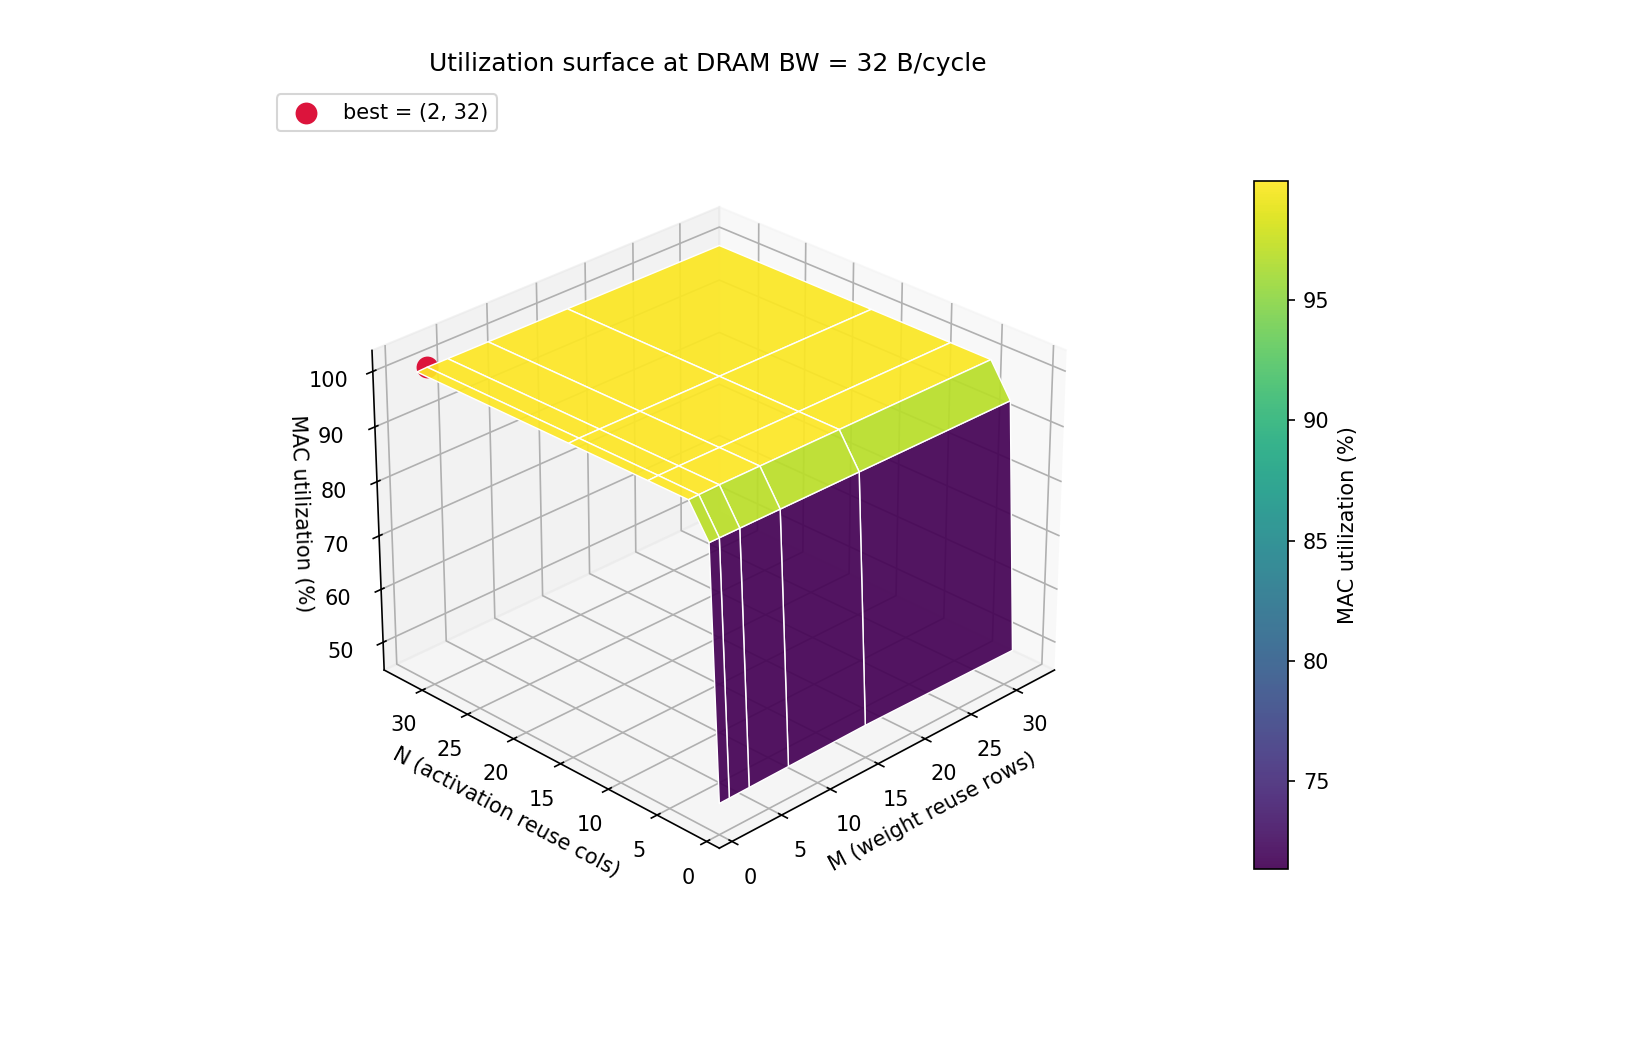
\includegraphics[width=\linewidth,height=.95\textheight,keepaspectratio]{figures/mn_utilization_surface_bw32.png}
    \caption{Derived MAC-utilization surface for the simplified notebook model at $32$ B/cycle DRAM bandwidth. It should be read as a qualitative reuse trend rather than an end-to-end utilization prediction.}
    \label{fig:mn-util-surface}
\end{figure}

\subsection{Measured Reuse-Policy Comparison}
% compare Naive, m2_n4, m2_n8, m4_n4, and m4_n8 using the measured blocked_mn_reuse_1024 results
% focus on cycles, bytes_transmitted, throughput, arithmetic intensity, and active/full-run utilization
% identify which policies reduce external traffic the most and which deliver the best end-to-end speedup
% this is the main measured comparison table/plot subsection

For cross-policy comparison, throughput is reported algorithmically as fixed GEMM FLOPs divided by total cycles. Unlike microarchitectural floating-point counts, which vary with how much accumulator traffic and other internal work each schedule generates, this measure stays invariant across schedules and therefore supports a cleaner end-to-end comparison. \Cref{tab:reuse-policy-comparison} shows that every blocked policy improves on the naive baseline in cycles, external traffic, and utilization.

\begin{table}[ht]
\centering
\small
\caption{Measured policy comparison. The naive row uses the tiled baseline from this evaluation; the $m8\_n32$ point uses the measured queue-size-4 run from the scratchpad-frontend queue sweep.}
\label{tab:reuse-policy-comparison}
\resizebox{\columnwidth}{!}{
\begin{tabular}{lrrrrrr}
\toprule
Policy & Cycles & Bytes & Algo tput & Ext. AI & Full util. & Active util. \\
 & (M) & (M) & (FLOP/cycle) & (FLOP/B) & (\%) & (\%) \\
\midrule
Naive & 22.93 & 268 & 93.66 & 8.00 & 4.57 & 45.07 \\
$m2\_n4$ & 15.36 & 218 & 139.78 & 9.85 & 6.83 & 78.05 \\
$m2\_n8$ & 12.95 & 210 & 165.86 & 10.24 & 8.10 & 87.67 \\
$m4\_n4$ & 13.25 & 218 & 162.07 & 9.85 & 7.91 & 78.05 \\
$m4\_n8$ & 11.97 & 210 & 179.38 & 10.24 & 8.76 & 87.67 \\
$m2\_n32$ & 12.67 & 203 & 169.51 & 10.56 & 8.28 & 96.60 \\
$m8\_n32$ & 11.22 & 203 & 191.44 & 10.56 & 9.35 & 96.60 \\
\bottomrule
\end{tabular}
}
\end{table}

Increasing activation reuse from $n=4$ to $n=8$ reduces VLS-visible traffic from 218M to 210M bytes and increases external arithmetic intensity from 9.85 to 10.24 FLOP/B, boosting the algorithmic throughput from 139.78 to 165.86 FLOP/cycle at $m2$ and from 162.07 to 179.38 FLOP/cycle at $m4$. At fixed $n=4$, increasing weight reuse from $m=2$ to $m=4$ leaves external traffic unchanged, but still cuts cycles from 15.36M to 13.25M, showing that extra resident weights improve overlap and feeding efficiency even when bytes moved per output tile do not change.

Extending activation reuse to $n=32$ reduces traffic again to 203M bytes and pushes the arithmetic intensity to 10.56 FLOP/B. However, reduced traffic alone is not enough to guarantee the best end-to-end result. The $m2\_n32$ point improves only modestly over $m2\_n8$, reaching 12.67M cycles and 169.51 FLOP/cycle, while $m8\_n32$ reaches the best measured point at 11.22M cycles and 191.44 FLOP/cycle, a 2.04$\times$ speedup over the 22.93M-cycle naive baseline. The comparison therefore shows that activation-side reuse provides the main traffic reduction, but weight-side residency still matters for turning that reduction into sustained compute utilization.

Despite the denser bursts, the full-run MAC utilization remains low in absolute terms. Even the best measured point, $m8\_n32$, reaches 96.60\% utilization only inside valid-MAC windows but averages 9.35\% over the full run. That gap shows that blocked reuse fixes array underfilling inside a burst far more effectively than it removes the long non-MAC phases around those bursts: preload, psum load/store, GSAU return handling, and scratchpad/vector-core service still dominate wall-clock time.

\subsection{Memory-System Sensitivity Under Reuse}
% use the measured m8_n32 scratchpad-frontend queue sweep as the sensitivity study
% show how performance changes as queue depth increases and where the benefit plateaus
% relate the cycle trend to gsau_rd_queue pressure and the remaining preload bottleneck
% keep any DRAM-burst discussion here only if it is backed by measured logs, not notebook intuition

The available scratchpad-frontend queue sweep was run at $m8\_n32$, which is an appropriate point for post-reuse sensitivity because it already sits near the best measured reuse setting. This lets us ask whether additional queueing capacity can remove the residual stalls that remain once reuse has already reduced external traffic per output tile.

\begin{figure}
    \centering
    \includegraphics[width=\linewidth,height=.95\textheight,keepaspectratio]{figures/cycles_vs_spad_frontend_queue_size.png}
    \caption{Un-throttling the system by increasing Scratchpad-to-Vector Core bandwidth}
    \label{fig:spad-fe-q-cycl}
\end{figure}

\Cref{fig:spad-fe-q-cycl} shows that increasing the queue size from 1 to 2 cuts total cycles from 15.54M to 12.66M, and increasing it again to 4 reduces cycles further to 11.22M. Beyond that point the returns are negligible: queue sizes 6 and 8 deliver 11.18M and 11.17M cycles, respectively.

\begin{figure}
    \centering
    \includegraphics[width=\linewidth,height=.95\textheight,keepaspectratio]{figures/gsau_rd_queue_vs_spad_frontend_queue_size.png}
    \caption{Feeding the systolic array by relaxing Scratchpad's Frontend}
    \label{fig:spad-fe-q-gsau}
\end{figure}

At \cref{fig:spad-fe-q-gsau}, over valid-MAC cycles, the average GSAU read-queue depth rises from 7.89 at queue size 1 to 13.76 at size 2 and 22.50 at size 4, then changes only slightly to 22.67 and 22.72 at sizes 6 and 8. Full-run MAC utilization follows the same trend, climbing from 6.75\% to 9.35\% by queue size 4 and then flattening. The active-window metric is less informative here because it stays tightly clustered around 96\% across the sweep: once a tile-GEMM reaches the array, the array is already nearly full. The improvement instead comes from shrinking the non-compute part of the schedule. Valid-MAC work stays essentially constant at about 1.09M cycles across queue sizes 1 through 8, so the 4.32M-cycle reduction from queue size 1 to 4 is almost entirely stall/support time removed from psum reload, return-path buffering, and accumulation flow control. Beyond queue size 4, the GSAU read queue is already deep enough to absorb most bursts, so larger queues add storage but do not materially increase the service rate of preload or accumulation support.

\subsection{Roofline Analysis}
% place the naive baseline and measured blocked policies on the roofline
% show the rightward shift from higher arithmetic intensity and the upward shift from higher measured throughput
% discuss which policies remain bandwidth-limited and whether any begin to approach the compute roof or knee
% use the roofline to connect the traffic reductions back to the observed speedups

\begin{figure}
    \centering
    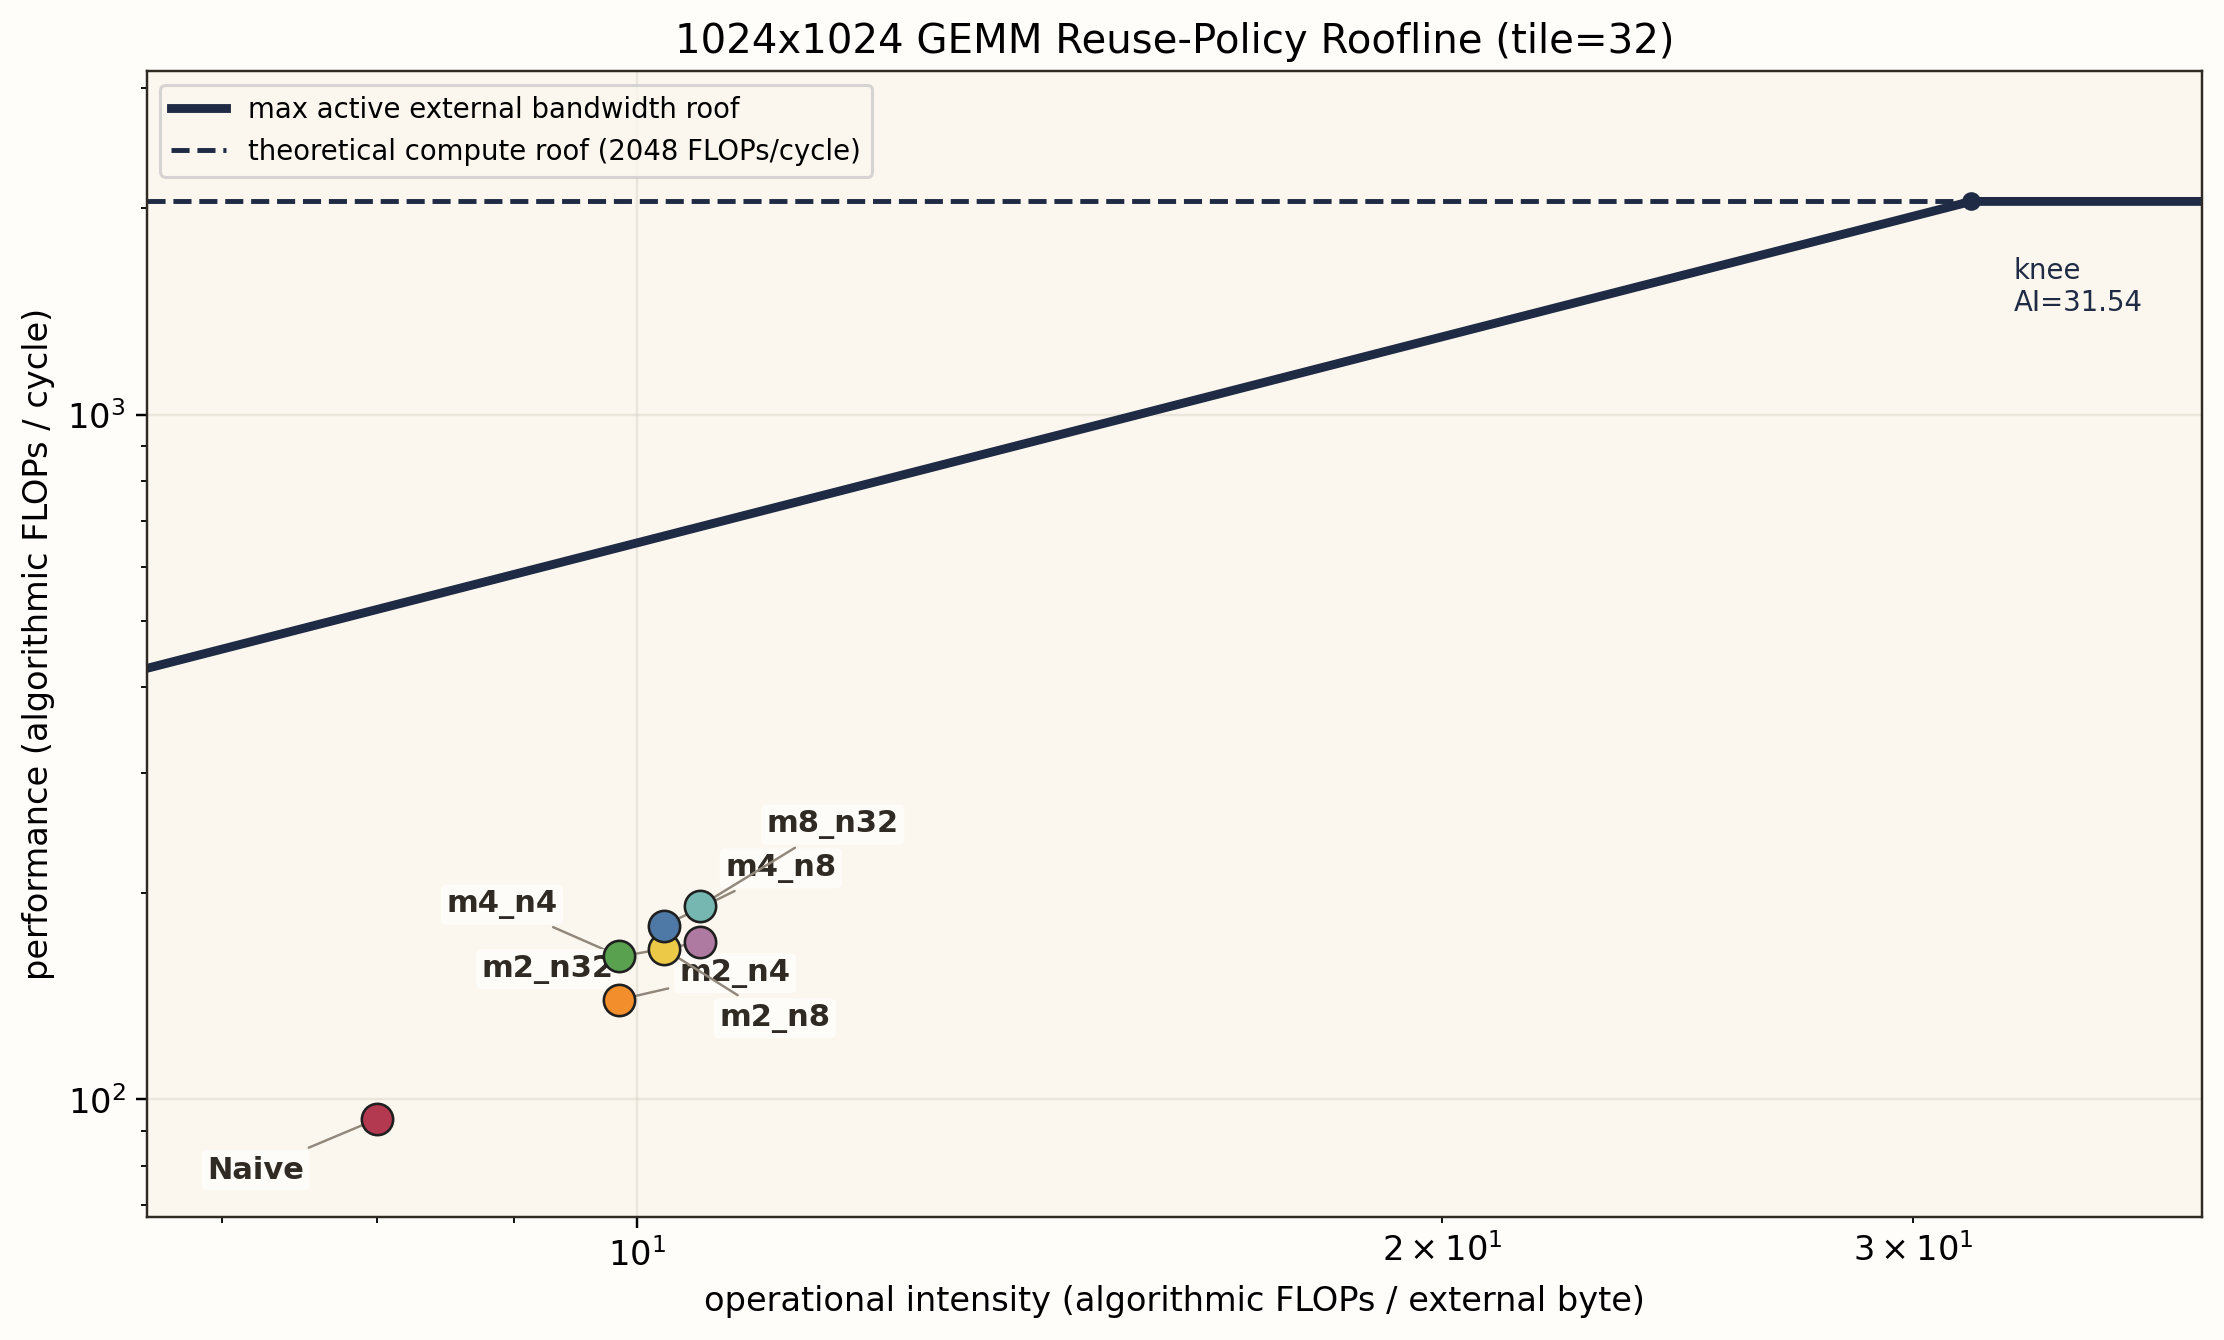
\includegraphics[width=\linewidth,height=.95\textheight,keepaspectratio]{figures/reuse_policy_roofline.png}
    \caption{Roofline plot for different tiling strategies, using $P(I)=\min(P_{\max}, B_{\max} I)$ with a systolic-array compute roof and an empirical active external-bandwidth roof.}
    \label{fig:roofline}
\end{figure}

\Cref{fig:roofline} is constructed from the standard roofline relation
$$
P(I) = \min(P_{\max}, B_{\max} I),
$$
where each plotted policy point uses the fixed algorithmic GEMM work for the numerator: $P = \frac{2N^3}{\text{cycles}}$ FLOP/cycle and $I = \frac{2N^3}{\texttt{bytes\_transmitted}}$ FLOP/B for the $1024\times1024$ GEMM. For this report, the compute roof is taken from the systolic array alone,
$$
P_{\max} = 2 \cdot \texttt{tile\_size}^2 = 2 \cdot 32^2 = 2048\ \text{FLOP/cycle},
$$
because a fully occupied $32\times32$ MAC array performs one multiply-accumulate per PE per cycle and each MAC counts as two floating-point operations. The bandwidth roof uses the maximum measured active external bandwidth across the compared runs, $B_{\max}=64.94$ B/cycle. This yields a roofline knee at about $\frac{2048}{64.94} \approx 31.5$ FLOP/B. If the model were extended to overlap vector-lane accumulation with systolic-array matmul and count that overlapped work in the same performance metric, then $P_{\max}$ would need to be redefined accordingly; the current roof uses only the matmul engine peak.

Under that construction, the naive baseline sits at roughly $(8.00\ \text{FLOP/B}, 93.66\ \text{FLOP/cycle})$. Moving to $m2\_n4$ and $m2\_n8$ shifts the operating point to the right as external bytes fall from 268M to 218M and then 210M, and upward as throughput rises to 139.78 and 165.86 FLOP/cycle. The $m4$ points show the complementary effect of weight residency: $m4\_n4$ and $m4\_n8$ have the same arithmetic intensities as the corresponding $m2$ points, but higher throughput, indicating that once bytes moved are fixed, additional resident weights improve how efficiently that traffic is converted into sustained compute.

The larger $n=32$ points continue this trend, reaching about 10.56 FLOP/B and 169.51 FLOP/cycle for $m2\_n32$ and 191.44 FLOP/cycle for $m8\_n32$. Even so, all of these points remain far below the 2048 FLOP/cycle compute roof and well left of the roofline knee at about 31.5 FLOP/B. The blocked policies therefore move the system in the right direction, but they do not bring it close to the compute roof. The measured gains remain bandwidth-limited improvements driven by traffic reduction and better overlap, not by any approach to peak arithmetic throughput.

\subsection{Evaluation Summary}
% summarize the baseline bottleneck, the effect of blocked reuse, and the new post-reuse limiter
% keep this to 3--4 direct takeaways tied to the measured results
% close by stating what the best measured policy demonstrates and what still prevents peak-compute operation

1- The tiled naive solution works correctly, but it is heavily preload- and accumulation-limited. Only about 10\% of total cycles fall inside valid-MAC windows, and even those windows fill the array to just 45.07\%, which is why the end-to-end MAC utilization is only 4.57\%.

2- Blocked reuse significantly reduces traffic and makes the compute bursts much denser. Compared to the naive solution, which generates 268M bytes of VLS-visible traffic, blocked policies reduce traffic first to 218M, then to 210M, and finally to 203M bytes while increasing throughput from 93.66 to a maximum of 191.44 FLOP/cycle and active-window MAC utilization from 45.07\% to 96.60\%.

3- Activation-side reuse reduces traffic more effectively than additional weight-side residency, but the latter remains important for sustaining higher throughput. The best measured point is $m8\_n32$ with queue size 4, reaching 11.22M cycles and a 2.04$\times$ speedup versus the naive baseline, but its full-run MAC utilization is still only 9.35\% because preload, psum reload/store, and queue/service overhead still consume roughly 90\% of total cycles.
% pre-silicon verification strategy: sw-hw co-design, validation against rtl
% 1024x1024 GEMM

\section{Conclusion and Future Work}
Atalla-Sim demonstrates that a custom cycle-level simulator can expose meaningful architectural bottlenecks before a complete RTL environment is available. In the $1024 \times 1024$ fp16 GEMM study, it showed that the naive tiled schedule is preload-limited, that blocked M/N reuse materially reduces VLS-visible traffic, and that the best measured configuration, $m8\_n32$ with scratchpad frontend queue size 4, reaches 11.22M cycles for a 2.04$\times$ speedup over the naive baseline. These results validate the simulator as a design-space exploration tool.

Although Atalla-Sim provides cycle-accurate visibility into queue pressure, overlap, and utilization, sweeping multiple parameters on the $1024 \times 1024$ GEMM still takes several hours, making broader exploration expensive and slows iteration of scheduling and memory ideas. Each new experiment currently depends on a handwritten harness that encodes staging policy, scratchpad placement, launch order, completion detection, and statistics collection in hundreds of lines of Python. This harness-centric workflow is hard to maintain, validate, and is too cumbersome to scaling to richer workloads.

The most important next step is therefore to repurpose the existing scheduler functional simulator into a cycle-accurate execution frontend for Atalla-Sim. The simulator should accept compiler-generated assembly files directly and run the same scheduled programs used by the software stack. That would remove a large amount of bespoke experiment code, align functional validation with performance evaluation, and make it practical to study more workloads than a single hand-assembled GEMM benchmark.

The current DRAM model is intentionally abstract, which is useful for early architectural exploration but limits the quality of memory-system conclusions. Hooking Ramulator into the system in place of this abstracted DRAM model would provide more realistic timing behavior and expose more informative performance metrics, including average memory access latency, read and write queue occupancy, row-buffer hit and miss behavior, bank-level parallelism, conflict-induced stalls, and sustained bandwidth under realistic request scheduling \cite{ramulator}.

With a compiler-driven execution path and higher-fidelity DRAM timing, Atalla-Sim can evolve from a useful prototype into a more scalable and more trustworthy platform for pre-silicon performance analysis.


% ---------- References ----------
\bibliographystyle{IEEEtran}
\bibliography{references}

\appendix

% \section{Teamwork}
% \input{sections/teamwork}

\end{document}
